\documentclass{article}

\usepackage{tikz}
\usepackage{pgfplots}
\pgfplotsset{compat=1.4} 


\begin{document}

\section{Question One}

``The progressiveness of difficult is adequate.''

\noindent
\begin{minipage}[t]{.5\textwidth}
\raggedright
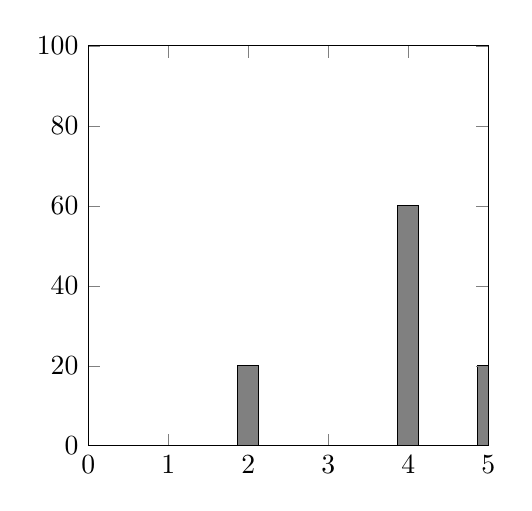
\begin{tikzpicture}
\begin{axis}[%
scale only axis,
width=2in,
height=2in,
xmin=0, xmax=5,
ymin=0, ymax=100,
axis on top]
\addplot[
  ybar,
  bar width=0.102874in, 
  fill=gray,
  draw=black] 
  plot coordinates{ 
    (1,0) (2,20)     (3,0) (4,60)     (5,20)
  };

\end{axis}
\end{tikzpicture}
\textit{Memory Stroop}
\end{minipage}% <---------------- Note the use of "%"
\begin{minipage}[t]{.5\textwidth}
\raggedleft
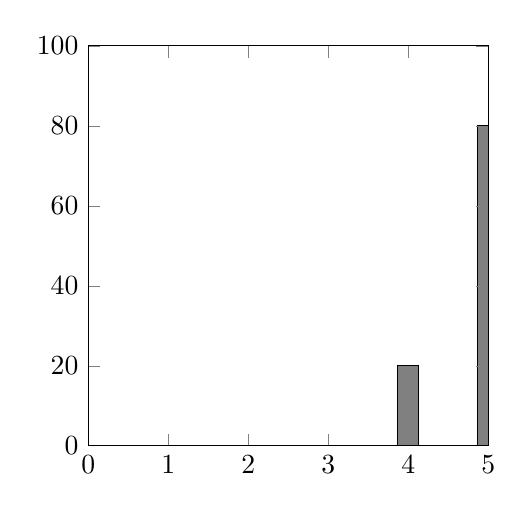
\begin{tikzpicture}
\begin{axis}[%
scale only axis,
width=2in,
height=2in,
xmin=0, xmax=5,
ymin=0, ymax=100,
axis on top]
\addplot[
  ybar,
  bar width=0.102874in, 
  fill=gray,
  draw=black] 
  plot coordinates{ 
    (1,0) (2,0)     (3,0) (4,20)     (5,80)
  };

\end{axis}
\end{tikzpicture}
\textit{Colors}
\end{minipage}


\section{Question Two}

``It is possible to understand the game rules.''

\noindent
\begin{minipage}[t]{.5\textwidth}
\raggedright
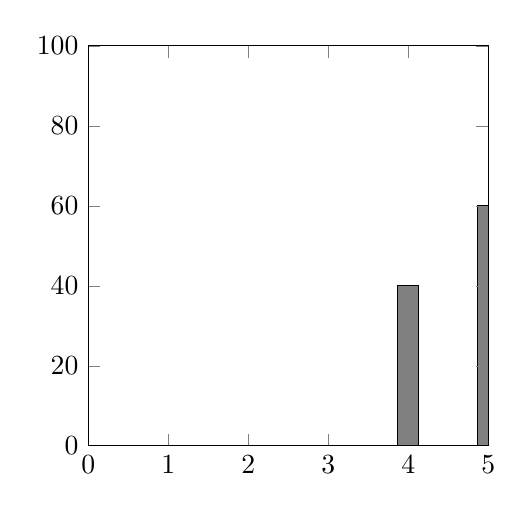
\begin{tikzpicture}
\begin{axis}[%
scale only axis,
width=2in,
height=2in,
xmin=0, xmax=5,
ymin=0, ymax=100,
axis on top]
\addplot[
  ybar,
  bar width=0.102874in, 
  fill=gray,
  draw=black] 
  plot coordinates{ 
    (1,0) (2,0)     (3,0) (4,40)     (5,60)
  };

\end{axis}
\end{tikzpicture}
\textit{Memory Stroop}
\end{minipage}% <---------------- Note the use of "%"
\begin{minipage}[t]{.5\textwidth}
\raggedleft
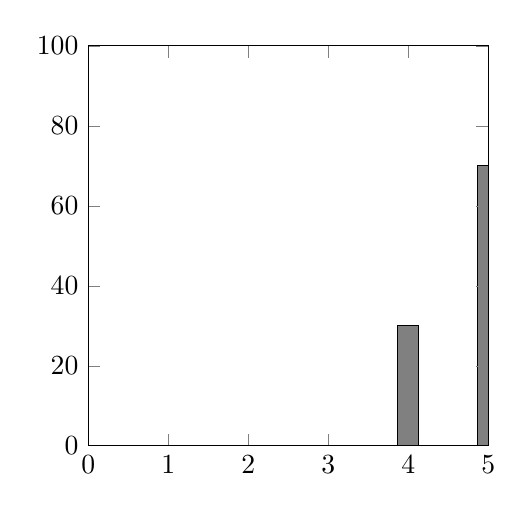
\begin{tikzpicture}
\begin{axis}[%
scale only axis,
width=2in,
height=2in,
xmin=0, xmax=5,
ymin=0, ymax=100,
axis on top]
\addplot[
  ybar,
  bar width=0.102874in, 
  fill=gray,
  draw=black] 
  plot coordinates{ 
    (1,0) (2,0)     (3,0) (4,30)     (5,70)
  };

\end{axis}
\end{tikzpicture}
\textit{Colors}
\end{minipage}
\newpage
\section{Question Three}

``The game is not functional, it is slow.''

\noindent
\begin{minipage}[t]{.5\textwidth}
\raggedright
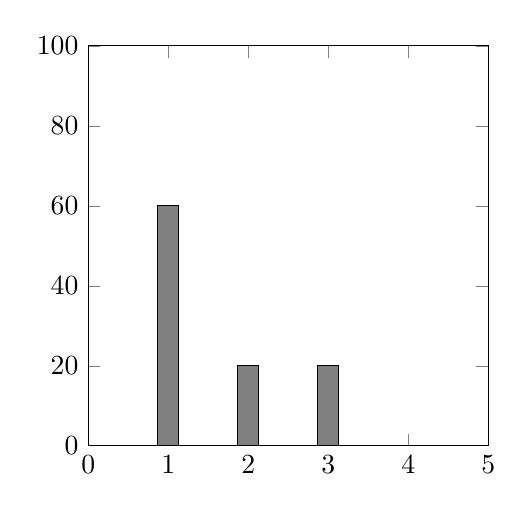
\begin{tikzpicture}
\begin{axis}[%
scale only axis,
width=2in,
height=2in,
xmin=0, xmax=5,
ymin=0, ymax=100,
axis on top]
\addplot[
  ybar,
  bar width=0.102874in, 
  fill=gray,
  draw=black] 
  plot coordinates{ 
    (1,60) (2,20)     (3,20) (4,0)     (5,0)
  };

\end{axis}
\end{tikzpicture}
\textit{Memory Stroop}
\end{minipage}% <---------------- Note the use of "%"
\begin{minipage}[t]{.5\textwidth}
\raggedleft
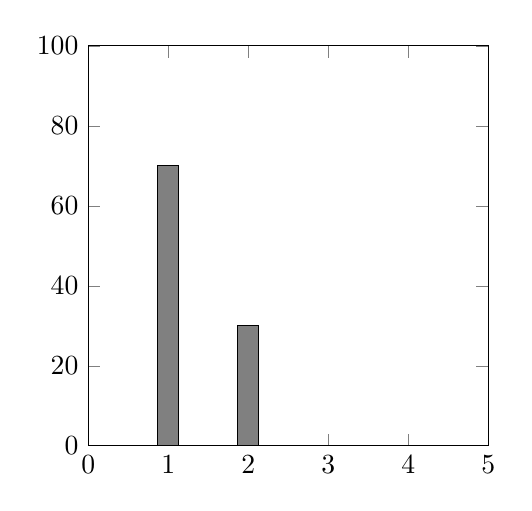
\begin{tikzpicture}
\begin{axis}[%
scale only axis,
width=2in,
height=2in,
xmin=0, xmax=5,
ymin=0, ymax=100,
axis on top]
\addplot[
  ybar,
  bar width=0.102874in, 
  fill=gray,
  draw=black] 
  plot coordinates{ 
    (1,70) (2,30)     (3,0) (4,0)     (5,0)
  };

\end{axis}
\end{tikzpicture}
\textit{Colors}
\end{minipage}

\section{Question Four}

``The proposed gamification is satisfactory.''

% 4

\noindent
\begin{minipage}[t]{.5\textwidth}
\raggedright
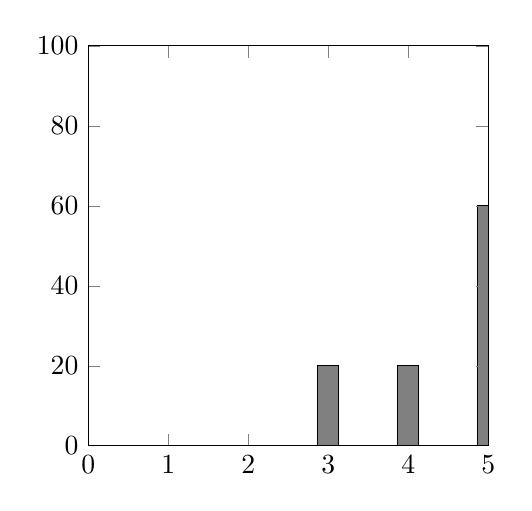
\begin{tikzpicture}
\begin{axis}[%
scale only axis,
width=2in,
height=2in,
xmin=0, xmax=5,
ymin=0, ymax=100,
axis on top]
\addplot[
  ybar,
  bar width=0.102874in, 
  fill=gray,
  draw=black] 
  plot coordinates{ 
    (1,0) (2,0)     (3,20) (4,20)     (5,60)
  };
\end{axis}
\end{tikzpicture}
\textit{Memory Stroop}
\end{minipage}% <---------------- Note the use of "%"
\begin{minipage}[t]{.5\textwidth}
\raggedleft
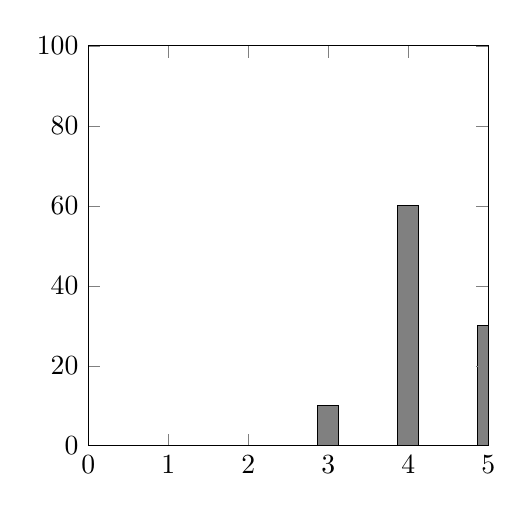
\begin{tikzpicture}
\begin{axis}[%
scale only axis,
width=2in,
height=2in,
xmin=0, xmax=5,
ymin=0, ymax=100,
axis on top]
\addplot[
  ybar,
  bar width=0.102874in, 
  fill=gray,
  draw=black] 
  plot coordinates{ 
    (1,0) (2,0)     (3,10) (4,60)     (5,30)
  };

\end{axis}
\end{tikzpicture}
\textit{Colors}
\end{minipage}

\newpage

\section{Question Five}

``The disposition of objects on screen is confuse.''

\noindent
\begin{minipage}[t]{.5\textwidth}
\raggedright
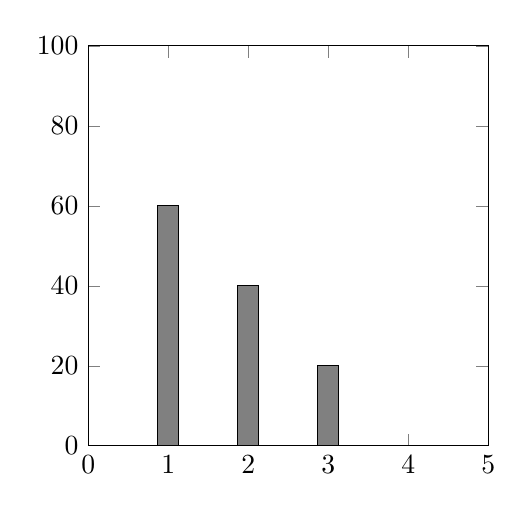
\begin{tikzpicture}
\begin{axis}[%
scale only axis,
width=2in,
height=2in,
xmin=0, xmax=5,
ymin=0, ymax=100,
axis on top]
\addplot[
  ybar,
  bar width=0.102874in, 
  fill=gray,
  draw=black] 
  plot coordinates{ 
    (1,60) (2,40)     (3,20) (4,0)     (5,0)
  };

\end{axis}
\end{tikzpicture}
\textit{Memory Stroop}
\end{minipage}% <---------------- Note the use of "%"
\begin{minipage}[t]{.5\textwidth}
\raggedleft
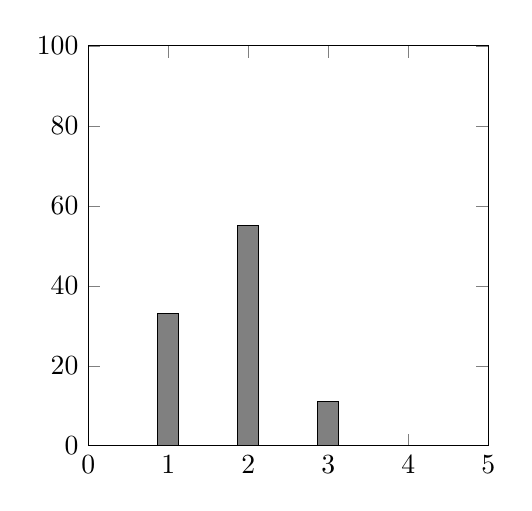
\begin{tikzpicture}
\begin{axis}[%
scale only axis,
width=2in,
height=2in,
xmin=0, xmax=5,
ymin=0, ymax=100,
axis on top]
\addplot[
  ybar,
  bar width=0.102874in, 
  fill=gray,
  draw=black] 
  plot coordinates{ 
    (1,33) (2,55)     (3,11) (4,0)     (5,0)
  };
\end{axis}
\end{tikzpicture}
\textit{Colors}
\end{minipage}


\section{Question Six}

``The game informs the player situation well.''

\noindent
\begin{minipage}[t]{.5\textwidth}
\raggedright
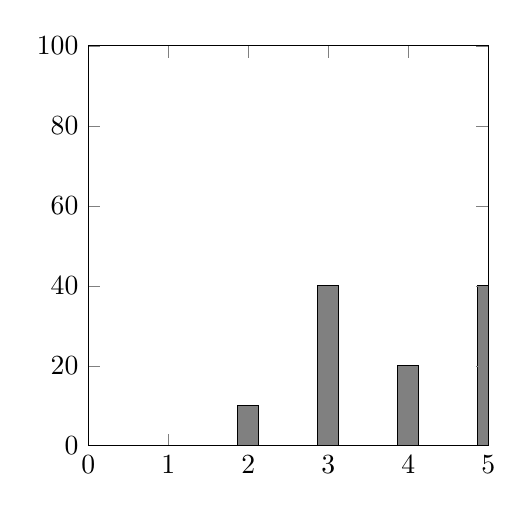
\begin{tikzpicture}
\begin{axis}[%
scale only axis,
width=2in,
height=2in,
xmin=0, xmax=5,
ymin=0, ymax=100,
axis on top]
\addplot[
  ybar,
  bar width=0.102874in, 
  fill=gray,
  draw=black] 
  plot coordinates{ 
    (1,0) (2,10)     (3,40) (4,20)     (5,40)
  };

\end{axis}
\end{tikzpicture}
\textit{Memory Stroop}
\end{minipage}% <---------------- Note the use of "%"
\begin{minipage}[t]{.5\textwidth}
\raggedleft
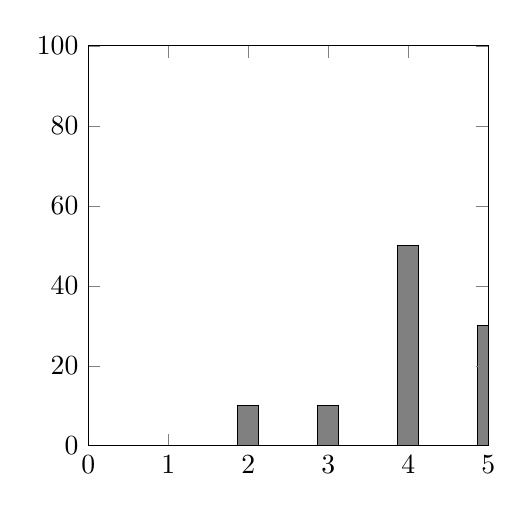
\begin{tikzpicture}
\begin{axis}[%
scale only axis,
width=2in,
height=2in,
xmin=0, xmax=5,
ymin=0, ymax=100,
axis on top]
\addplot[
  ybar,
  bar width=0.102874in, 
  fill=gray,
  draw=black] 
  plot coordinates{ 
    (1,0) (2,10)     (3,10) (4,50)     (5,30)
  };

\end{axis}

\end{tikzpicture}
\textit{Colors}
\end{minipage}

\newpage

\section{Question Seven}

``The screen sequence is confuse.''

\noindent
\begin{minipage}[t]{.5\textwidth}
\raggedright
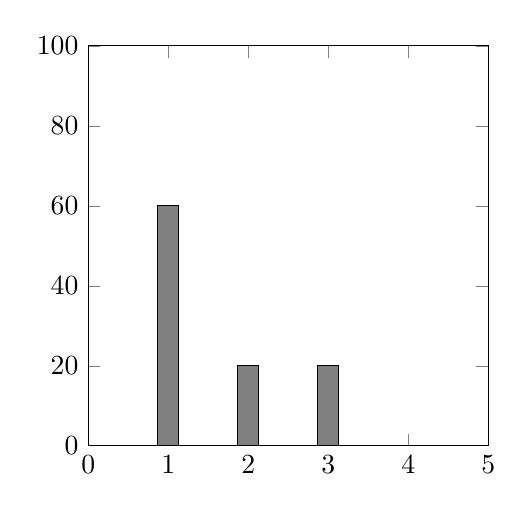
\begin{tikzpicture}
\begin{axis}[%
scale only axis,
width=2in,
height=2in,
xmin=0, xmax=5,
ymin=0, ymax=100,
axis on top]
\addplot[
  ybar,
  bar width=0.102874in, 
  fill=gray,
  draw=black] 
  plot coordinates{ 
    (1,60) (2,20)     (3,20) (4,0)     (5,0)
  };

\end{axis}
\end{tikzpicture}
\textit{Memory Stroop}
\end{minipage}% <---------------- Note the use of "%"
\begin{minipage}[t]{.5\textwidth}
\raggedleft
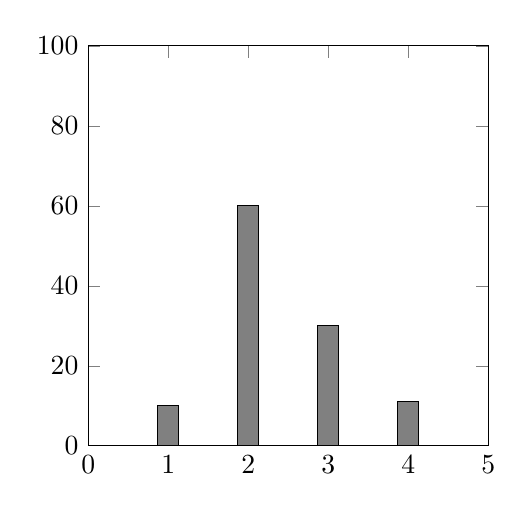
\begin{tikzpicture}
\begin{axis}[%
scale only axis,
width=2in,
height=2in,
xmin=0, xmax=5,
ymin=0, ymax=100,
axis on top]
\addplot[
  ybar,
  bar width=0.102874in, 
  fill=gray,
  draw=black] 
  plot coordinates{ 
    (1,10) (2,60)     (3,30) (4,11)     (5,0)
  };

\end{axis}
\end{tikzpicture}
\textit{Colors}
\end{minipage}


\section{Questions Eight and Nine -- Bivalent Questions}


``Have you needed some help to understand the game?''

\noindent
\begin{minipage}[t]{.5\textwidth}
\raggedright
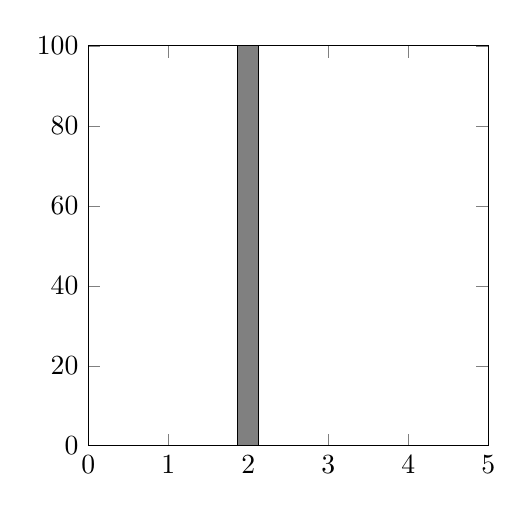
\begin{tikzpicture}
\begin{axis}[%
scale only axis,
width=2in,
height=2in,
xmin=0, xmax=5,
ymin=0, ymax=100,
axis on top]
\addplot[
  ybar,
  bar width=0.102874in, 
  fill=gray,
  draw=black] 
  plot coordinates{ 
    (1,0) (2,100)
  };

\end{axis}
\end{tikzpicture}
\textit{Memory Stroop}
\end{minipage}% <---------------- Note the use of "%"
\begin{minipage}[t]{.5\textwidth}
\raggedleft
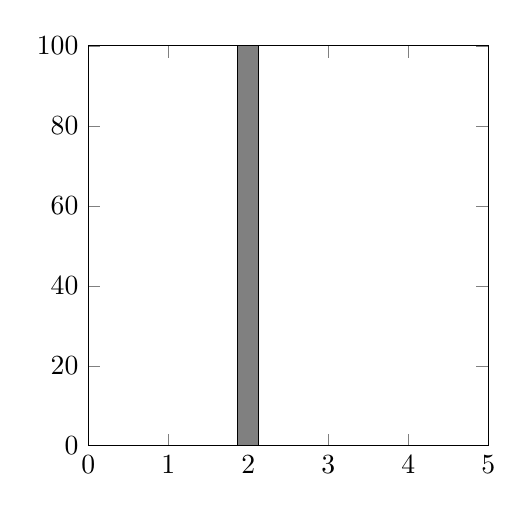
\begin{tikzpicture}
\begin{axis}[%
scale only axis,
width=2in,
height=2in,
xmin=0, xmax=5,
ymin=0, ymax=100,
axis on top]
\addplot[
  ybar,
  bar width=0.102874in, 
  fill=gray,
  draw=black] 
  plot coordinates{ 
    (1,0) (2,100)
  };

\end{axis}
\end{tikzpicture}
\textit{Colors}
\end{minipage}


``Does the game present any error?''

\noindent
\begin{minipage}[t]{.5\textwidth}
\raggedright
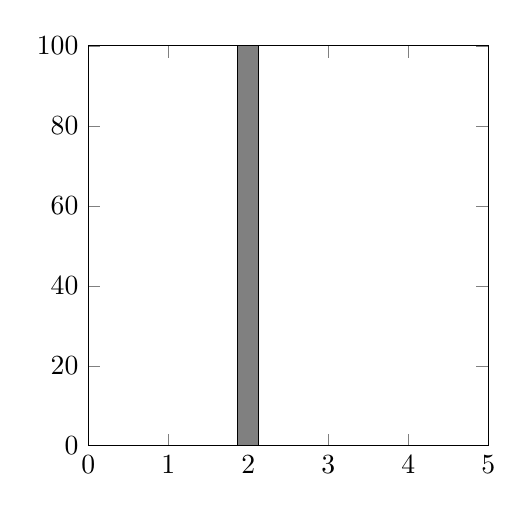
\begin{tikzpicture}
\begin{axis}[%
scale only axis,
width=2in,
height=2in,
xmin=0, xmax=5,
ymin=0, ymax=100,
axis on top]
\addplot[
  ybar,
  bar width=0.102874in, 
  fill=gray,
  draw=black] 
  plot coordinates{ 
    (1,0) (2,100)
  };

\end{axis}
\end{tikzpicture}
\textit{Memory Stroop}
\end{minipage}% <---------------- Note the use of "%"
\begin{minipage}[t]{.5\textwidth}
\raggedleft
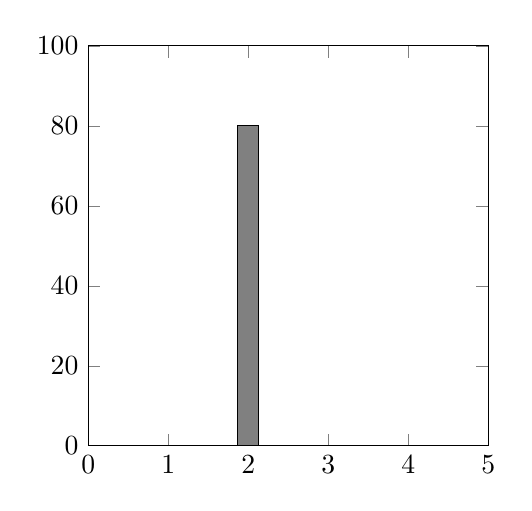
\begin{tikzpicture}
\begin{axis}[%
scale only axis,
width=2in,
height=2in,
xmin=0, xmax=5,
ymin=0, ymax=100,
axis on top]
\addplot[
  ybar,
  bar width=0.102874in, 
  fill=gray,
  draw=black] 
  plot coordinates{ 
    (1,0) (2,80)
  };

\end{axis}
\end{tikzpicture}
\textit{Colors}
\end{minipage}

\end{document}